% SLOGAN: This chapter formally introduces "the maintenance view."
% Sticky sentence: "Categories are real because they are maintained."
% See notes/book-slogans.md for the book-wide slogan strategy.

\chapter{Categories without essences}
\label{ch:kinds-without-essences}

\epigraph{You should consider that the essential art of civilization is maintenance.}{— Pete Seeger, quoted in \citet{brand2024}}

Part I raised a question: if categories aren't defined by essences, what makes them real? The answer this chapter develops is simple: categories are real because they are maintained. This is the \ixs{maintenance view}\term{maintenance view}.

The word \enquote{maintenance} is chosen deliberately. Stewart Brand's recent work on infrastructure, buildings, and software makes a point that applies equally to language: maintenance isn't just preventing breakdown; it's the whole process of keeping something going \citep{brand2024}. Monitoring, repair, renewal, adaptation~-- these are what keep bridges standing and cities functioning. Brand's insight is that we systematically undervalue maintenance because its successes are invisible: a well-maintained system just \emph{works}, and we notice only when it fails.

Linguistic categories are like this. Grammatical categories are the cleanest place to see it, but the same maintenance logic shows up in phoneme contrasts and in register conventions. When the system functions smoothly, the maintenance is invisible. We notice it only when it fails or when we look specifically at the seams.

Stated as a commitment:

\begin{quote}
\textbf{HPC commitment:} A category is real when (a) it is associated with a robust cluster of properties, and (b) there exist processes that tend to produce and stabilize that cluster across the relevant range of contexts, yielding projectible generalisations.
\end{quote}

The commitment is designed to be vulnerable. It can fail: the cluster can be too thin to support induction; the apparent cluster can be a measurement artefact; or the cluster can be maintained by multiple distinct processes, in which case the label covers several kinds rather than one. Those are empirical diagnoses, not definitional loopholes.

The idea of maintenance as constitutive~-- not just preservative~-- comes from philosophy of biology. Species aren't defined by genetic essences~-- no checklist of necessary and sufficient conditions separates one species from another. But species are real. They support induction, figure in explanations, persist across time. What makes them real is not a shared essence but a shared causal history: mechanisms of reproduction, selection, and development that keep certain properties clustering together.

\ixnq{Boyd, Richard}Richard Boyd called these homeostatic property cluster (HPC) kinds~-- or just HPC kinds \citep{boyd1991,boyd1999}. The name is technical but its parts are revealing. \emph{Stasis}: standing, position~-- the cluster \emph{stays} in place, maintained by ongoing processes. \emph{Homeo}: same, similar~-- when disturbed, the cluster tends to return to the \emph{same} configuration, not just any stable state. A homeostatic system doesn't merely persist; it self-corrects. Perturb a species' genome and selection pushes back toward the original distribution. Isolate a population and reproductive barriers emerge that restore the clustering. The name captures both the \emph{staying} and the \emph{sameness}~-- stability is not just inertia but active return.

Think of a spinning top. It stays upright not because it's rigid but because it's moving. The spin resists perturbation~-- push it slightly and gyroscopic forces bring it back. Stop the spin and the top falls. Homeostatic kinds are like this: their stability is dynamic, not static. What keeps the cluster clustered is not a fixed structure but an ongoing process. If this stability is real, it should have measurable signatures: judgment variance should spike near category boundaries; innovation should stall when it encounters alignment resistance; diffusion rates should differ for items that comply with the basin versus those that violate it. Those predictions are developed in §\ref{subsec:4:falsification}.

\ixnq{Millikan, Ruth}Ruth Millikan provides deeper metaphysical grounding: \enquote{Anything with a structure that tends actively to maintain or reconstitute itself over time~[\ldots] maintains or increases its own kind while depleting materials and resources for constituting other kinds} \citep[ch.~1, p.~17]{millikan2017}. Self-maintaining structures crowd out competitors. The limited variety we observe~-- discrete species rather than a continuum of forms, distinct linguistic categories rather than undifferentiated distribution~-- reflects not the prior structure of reality but the selective survival of self-stabilizing clusters. The asymmetry is counterfactual: maintained clusters are resilient in characteristic ways~-- perturb them and they tend to return; remove the maintenance and they dissolve. Merely convenient groupings lack this resilience. That's what distinguishes HPC kinds from bookkeeping.

\begin{figure}[t]
\centering
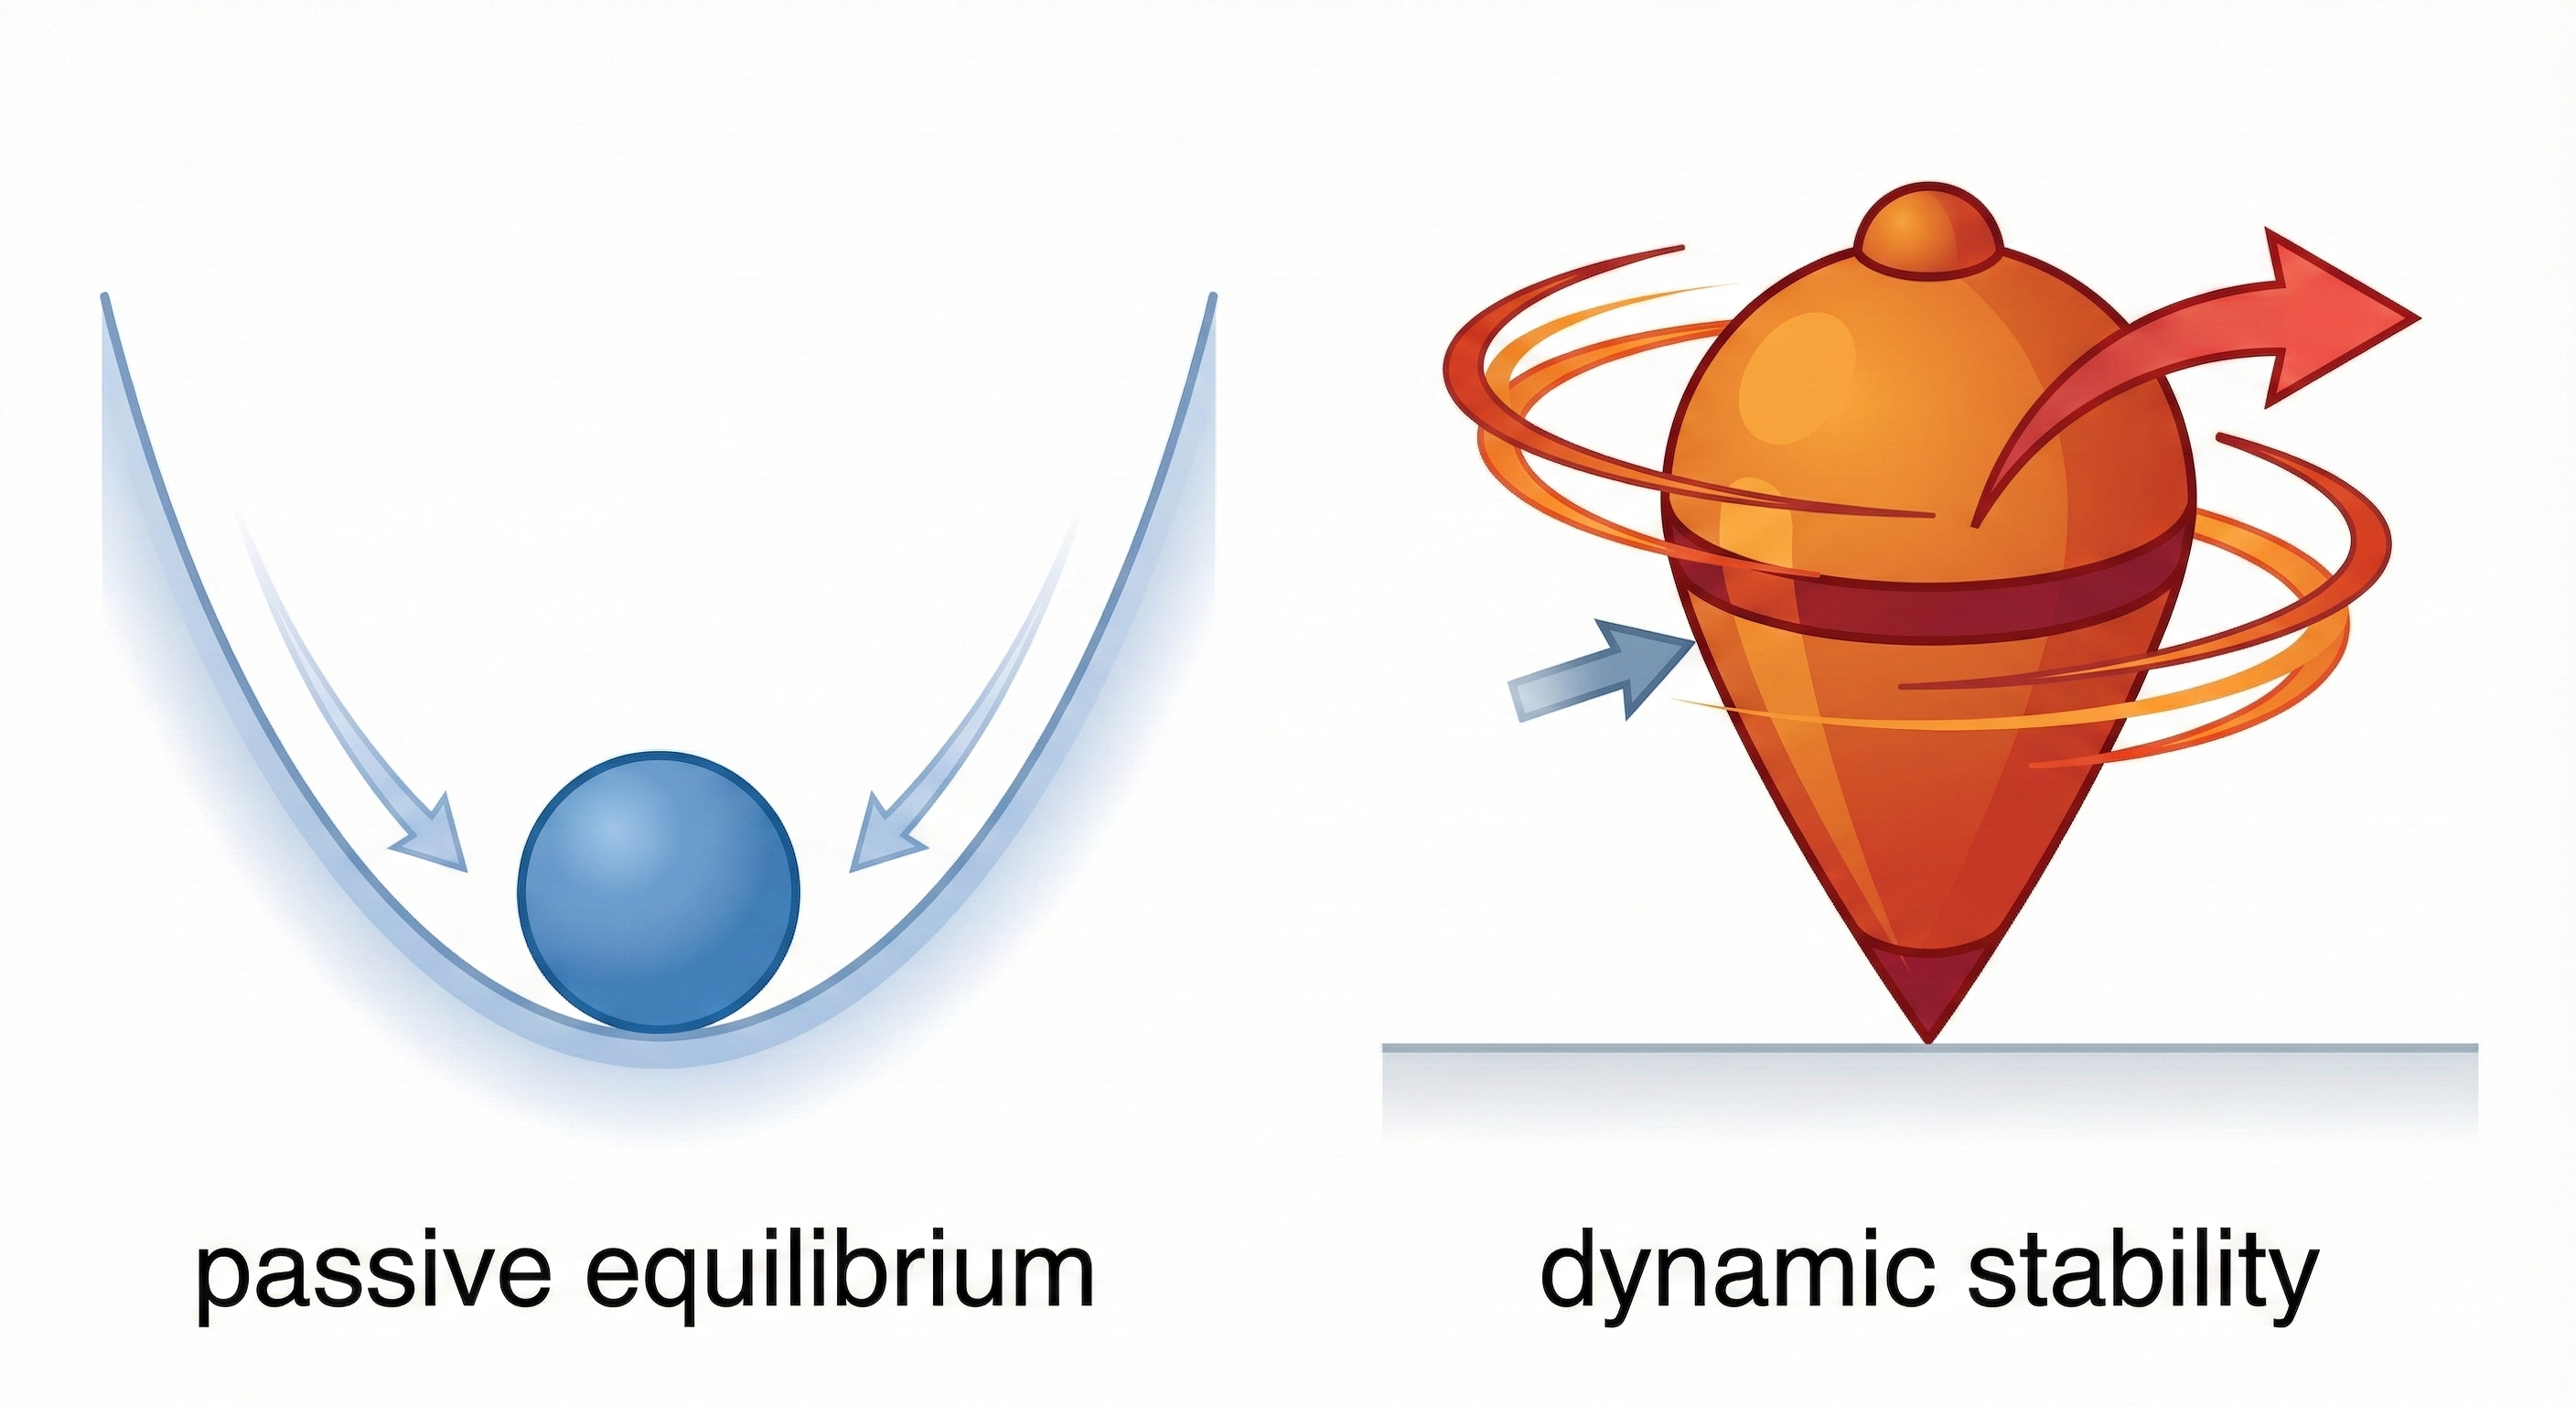
\includegraphics[width=0.75\textwidth]{figures/4.top-vs-ball.png}
\caption{Two kinds of stability. Left: a ball at the bottom of a valley is in passive equilibrium~-- it settles where gravity deposits it. Right: a spinning top maintains dynamic stability~-- the spin actively resists perturbation, and when pushed, gyroscopic forces push back. Homeostatic property cluster kinds are like the top: their stability is achieved through ongoing processes, not through static structure.}
\label{fig:top-vs-ball}
\end{figure}

And the maintenance needn't be entirely external. Some of the stability arises from reciprocal reinforcement among the clustered properties themselves. Recall \textit{Smilodon} and \textit{Thylacosmilus} from §\ref{sec:2:a-parallel} (Figure~\ref{fig:convergent-morphology}): their massive canines, powerful forelimbs, solitary hunting, and apex-predator niche aren't accidentally co-present. They are causally interlocking~-- each makes the others more likely, more stable, more resistant to drift. Large canines require the musculature to wield them; ambush predation requires the solitude to stalk; apex status requires the whole package. The cluster is a self-stabilizing network, embedded in broader developmental, ecological, and transmission dynamics. This is the reflexive dimension of homeostasis: the properties, by virtue of being those properties, participate in maintaining the cluster.

The question of why creatures categorize at all~-- why cognition traffics in discrete kinds rather than continuous similarity gradients~-- is beyond this book's scope. The short answer is evolutionary: organisms that tracked projectable regularities outcompeted those that didn't \citep{quine1969}. \citet{millikan1984} develops this insight into a comprehensive theory of biological function, while developmental work by \citet{gelman1987} shows that the tendency to essentialize categories appears very early in childhood, suggesting a cognitive default that education must work against rather than a learned strategy.


\section{From species to categories}
\label{sec:4:species-to-categories}

The biological parallel isn't decorative. Species and linguistic categories face the same philosophical problem: both look like natural kinds~-- they support induction, figure in explanations, persist across time~-- but neither has an essence in the classical sense. No genetic sequence is necessary and sufficient for tigerdom; no morphosyntactic property is necessary and sufficient for nounhood. But tigers are real, and so are nouns. The question is how.

Boyd's answer for species was that the clustering does the epistemic work while the mechanisms explain the clustering. Tigers share properties~-- striped fur, carnivorous diet, solitary hunting, particular vocalizations~-- not because these properties define \mention{tiger} but because the mechanisms of reproduction, development, and selection keep them bundled together. The properties vary; not every tiger has all of them. But they cluster reliably enough that learning about one tiger tells you something about others. That's what makes \mention{tiger} projectible~-- able to support inductive inference~-- even without a definition.

The same logic applies to grammatical categories. Nouns share properties~-- they head noun phrases, occur with determinatives, inflect for number, denote entities~-- not because these properties define \term{noun} but because the mechanisms of acquisition, entrenchment, and transmission keep them bundled. The properties vary; not every noun has all of them. But they cluster reliably enough that learning the category \term{noun} tells you something about how unfamiliar nouns will behave.

Ruth Millikan's work on \term{copied kind}s sharpens the parallel \citep{millikan1984,millikan2017}. A copied kind is a category whose members are produced from each other or from a common template~-- they share properties because they share a lineage, not because they share an essence. Biological species are copied kinds: each organism is a copy (with variation) of its parents. Artefacts like screwdrivers are copied kinds: each is produced from a template (with variation) that was itself copied from earlier templates.

Grammatical categories are copied kinds par excellence. Each generation doesn't invent nouns from scratch; children copy the category from their input, with variation, and pass it on. The properties cluster because the copying is high-fidelity enough to preserve them. The variation accumulates because no copying is perfect. The category persists because the lineage persists~-- an unbroken chain of transmission from speaker to speaker across millennia. Khalidi calls such history-defined kinds \term{etiological kind}s and defends their status as genuine natural kinds \citep[106--112]{khalidi2013}.

Millikan's later work on \term{unicept}s sharpens the point \citep[ch.~3]{millikan2017}. A unicept tracks sameness through multiple fallible methods~-- we recognize a friend by face, voice, gait, or handwriting, with none privileged as definitional. The same structure applies to grammatical categories: we identify nouns through plural morphology, determiner compatibility, argument positions, semantic features, and more. None of these diagnostics is the \enquote{real} definition of nounhood; they are all ways of tracking the same maintained cluster. The category is what the diagnostics converge on, not what any single diagnostic defines.

The neural evidence is suggestive. \textcite{Fedorenko2024naturalkind} argue that the brain's language network~-- frontal and temporal regions that respond selectively to linguistic meaning~-- exhibits functional cohesion across diverse tasks despite anatomical variability across individuals. This is evidence that stability-with-heterogeneity is respectable in cognitive science: natural-kind talk can apply where functional profile is stable even when anatomical substrate varies. The result is best treated as an existence proof rather than direct confirmation of the specific mechanisms developed here~-- but it shows that HPC-style kinds aren't peculiar to biology.

This is what makes the biological parallel load-bearing rather than merely illustrative. The mechanisms maintaining species cohesion~-- reproduction, gene flow, selection, developmental constraint~-- have genuine analogues in language. Not identical mechanisms, but mechanisms playing the same structural role: keeping properties clustered, filtering variation, stabilizing the kind across time.

William Croft makes the parallel explicit: languages are \enquote{populations of utterances}, and linguistic variants compete in speaker communities much as phenotypes compete in biological populations \citep{croft2000}. Salikoko Mufwene takes the analogy further, comparing languages to viruses rather than organisms~-- they depend on hosts (speakers), multiple can coexist in one host, and they exchange material (borrowing) more readily than species do \citep{mufwene2001}. The analogy is imperfect but productive: it highlights that linguistic change operates via interactions in a population, not by reference to an immutable type.

\begin{table}[t]
\centering
\caption{Parallel mechanisms in biology and grammar}
\label{tab:parallel-mechanisms}
\begin{tabular}{@{}lll@{}}
\toprule
\textbf{Function} & \textbf{Biological mechanism} & \textbf{Linguistic mechanism} \\
\midrule
Transmission & Reproduction & Acquisition \\
Filtering & Natural selection & Communicative success \\
Cohesion & Gene flow & Interactive alignment \\
Constraint & Development & Processing limitations \\
Attraction & Ecological niche & Functional pressure \\
\bottomrule
\end{tabular}
\end{table}

Table~\ref{tab:parallel-mechanisms} sketches the correspondences.\footnote{These are functional analogues, not homologues: the mechanisms occupy the same position in an explanatory structure without sharing causal architecture. Analogy is scientifically respectable; the parallel is load-bearing but not a claim of identity.} Not every detail maps, and that's fine. The claim isn't that language \emph{is} biology but that the same style of explanation works: mechanism-based, historical, non-essentialist. What maintains the clustering matters more than what defines the category.


\section{What mechanisms mean}
\label{sec:4:mechanisms}

\term{Mechanism} is doing a lot of work here, so I should say briefly what I mean. By \term{mechanism} I mean an empirically tractable process with a characteristic signature under perturbation: change the inputs in a targeted way, and you can predict (within noise) the direction and timescale of the system's response. The mechanisms maintaining linguistic categories aren't mysterious: they're the processes that usage-based linguistics has been studying for decades (statistical learning, exemplar storage, analogical extension, routinization). When I say mechanisms \enquote{maintain} categories, I don't mean they keep categories frozen; maintenance includes change. A well-maintained building gets renovated; a well-maintained codebase gets refactored. The point is that the system keeps functioning, not that it stays identical. The detailed treatment of what makes a mechanism substantive rather than decorative~-- the perturbation criterion~-- comes in §\ref{subsec:4:mechanisms-not-metaphors}.

But how far does this constructive, on-the-fly view extend? A more radical position has recently emerged. \textcite{ambridge2020radical} argues that categories like \term{noun} and \term{verb} are not stored anywhere~-- not as essences, not as prototypes, not as schemas. Speakers store only individual utterances; the categories are emergent patterns, visible to the analyst but not represented in the mind. His analogy is the honeycomb: hexagonal structure is a real feature of beehives, but no bee represents hexagons. The structure emerges from the local behaviours of many bees following simple rules. \term{Noun}, on this view, is the linguistic honeycomb~-- real enough to describe, but not internally represented.

The analogy is useful but the conclusion doesn't follow. What makes the honeycomb real is not that bees lack hexagon-concepts; it's that the local behaviours~-- cell construction, wax physics, spatial constraints~-- reliably produce and maintain the hexagonal pattern. The structure persists because the mechanisms persist. This is exactly the HPC claim. Ambridge's ``radical exemplar'' model identifies the mechanisms~-- analogical generalisation across stored tokens~-- without recognizing that those mechanisms are what maintains the category as a real kind. The disagreement is about whether ``emergent'' means ``less than real.'' HPC says no: emergent patterns can constitute genuine kinds, provided the mechanisms that produce them operate reliably. Hexagons are real. So are nouns.


\section{The mechanisms themselves}
\label{sec:4:the-mechanisms}

Let me name the mechanisms concretely. This isn't an exhaustive list~-- Chapter~\ref{ch:stabilizers} develops a more detailed treatment~-- but it's enough to show that \enquote{mechanisms maintain categories} isn't hand-waving.

\subsection{Acquisition}
\label{subsec:4:acquisition}

Children acquire grammatical categories without being taught definitions. No parent explains that nouns are words that can be preceded by determinatives and followed by plural suffixes. Yet children converge on category systems that are highly similar to their parents'~-- not identical in every detail, since languages with different inventories produce different category structures, but similar at the level of major recurrent clusters. This convergence happens reliably, across cultures, in just a few years~-- a feat that explicit definition struggles to replicate.

How? Not by innate specification~-- that just relocates the essence to the genome and doesn't explain why categories vary across languages. The HPC answer is that children track statistical regularities that reflect the underlying mechanisms. They acquire categories by being sensitive to the pressures that maintain them.

The evidence is strong. Distributional learning~-- tracking which words occur in which contexts~-- is sufficient to induce grammatical categories from raw input \citep{redington1998,mintz2003,piantadosi2024,kallini2024}. Infants are sensitive to these distributions from early in the first year \citep{gomez2000}. The categories children induce match adult categories not because children have innate category templates but because the same distributional patterns that define adult categories are present in child-directed speech.

Acquisition is a mechanism of maintenance because it transmits categories across generations. Each child who learns \term{noun} from input and then uses nouns in ways the next generation can learn from keeps the category alive. The mechanism is imperfect~-- children don't reproduce their parents' grammars exactly~-- and this imperfection is itself important. Variation enters through acquisition; selection operates on that variation; categories evolve. But evolution isn't dissolution. The category persists because acquisition is reliable enough, even though it isn't perfect.

\subsection{Entrenchment}
\label{subsec:4:entrenchment}

Frequency matters. High-frequency items are processed faster, stored more robustly, and resist analogical pressure more strongly than low-frequency items \citep{bybee2006,diessel2007}. This is \ixsq{entrenchment}entrenchment: the deepening of mental representations through repeated use.

Entrenchment maintains categories by anchoring them. The most frequent nouns~-- \mention{thing}, \mention{time}, \mention{way}, \mention{people}~-- are processed automatically, without conscious categorisation. They are the bedrock of the category, the items that every speaker agrees on, the deep-basin anchors around which less frequent items cluster. Change the behaviour of \mention{thing} and you change what \term{noun} means. This is vanishingly unlikely. \mention{Thing} is so entrenched that changing it is nearly impossible~-- it would require shifting the habits of every English speaker simultaneously.

The skewed distribution isn't incidental~-- it's functional. \citet{wolters2024zipfian} showed that Zipfian input distributions facilitate children's word learning even in isolation tasks where cross-situational inference isn't required. High-frequency items serve as scaffolds: once entrenched, they provide stable reference points for acquiring lower-frequency forms. The very shape of natural language input is itself a stabilizer.

High-frequency items also grammaticalize faster. The path from lexical verb to auxiliary~-- \mention{will}, \mention{going to}, \mention{have to}~-- runs through frequent, semantically general items. Low-frequency items don't grammaticalize because they're not processed often enough to undergo the phonetic reduction and semantic bleaching that grammaticalization requires. The category \term{auxiliary} exists because entrenchment creates a basin of attraction: items that enter the basin get pulled toward the prototype; items outside it stay lexical.

Entrenchment also determines which syntactically well-formed expressions count as established in context. In English, the way to ask about someone's age is \mention{How old are you?}, with the response \mention{I'm forty} or \mention{I'm forty years old}. The calque from French would be \mention{What age do you have?} and \mention{I have forty years.} These clauses violate no syntactic rules of English, but the first set is entrenched for age-reporting and the second is not. As a result, the second set is constructionally misaligned for that functional slot~-- though \mention{I have forty years} is perfectly fine as a response to a query about time until retirement. The appropriateness of an expression can depend on its entrenchment within a particular functional slot, not just its structural well-formedness.

\subsection{Interactive alignment}
\label{subsec:4:alignment}

Speakers accommodate to each other. In conversation, interlocutors converge on lexical choices, syntactic structures, even phonetic details \citep{pickering2004,garrod2009}. This is \ixs{interactive alignment}\term{interactive alignment}: the tendency to match your speech to your interlocutor's.

Alignment maintains categories by enforcing community-wide coherence. If I use \mention{adult} as a verb and you accommodate, we've both reinforced the verb use. If you resist~-- if you pointedly say \mention{be responsible} instead~-- you've exerted pressure against the innovation. Either way, the interaction shapes subsequent usage. Multiply this by millions of conversations and you get a distributed mechanism for maintaining shared norms.

The alignment needn't be conscious. Most accommodation is automatic, below the level of awareness. Speakers don't decide to match their interlocutors' syntax; they just do. This automaticity makes alignment a powerful stabilizing force. Categories persist not because speakers explicitly agree on them but because speakers implicitly coordinate, conversation by conversation, year by year.

\subsection{Iterated transmission}
\label{subsec:4:transmission}

Language is transmitted imperfectly across generations. Children don't reproduce their parents' grammars exactly; each generation introduces variation. You might expect this imperfection to degrade structure~-- random errors accumulating until categories dissolve into noise. But the opposite happens. Structure emerges.

Simon Kirby and colleagues demonstrated this experimentally \citep{kirby2008,kirby2015compression}. Participants learned an artificial language~-- nonsense words paired with meanings~-- and then reproduced it for the next \enquote{generation.} The initial language was arbitrary: no pattern connected form to meaning. By generation ten, the language had become compositional~-- word parts systematically encoded meaning components. Structure emerged from the transmission process itself, as learnable variants outcompeted arbitrary ones.

The mechanism is a filter. Not all variants survive transmission equally. Easy-to-learn variants get reproduced faithfully; hard-to-learn variants get distorted or lost. Over generations, this filtering selects for systematicity. Languages become more learnable because learnable languages survive transmission; unlearnable ones don't.

For grammatical categories, the implication is direct. Categories that are easy to acquire~-- categories with clear distributional signatures, consistent morphological marking, coherent semantic cores~-- survive transmission better than categories without these properties. The categories we observe today are the residue of this filtering process, iterated across thousands of generations. They're structured because only structured categories could have survived.

But transmission isn't the only route. \citet{raviv2019structure} showed that compositional structure can emerge within a single generation when communities include multiple interaction partners and an expanding meaning space. The key isn't generational succession per se~-- it's the presence of compressibility pressure and communicative feedback. Transmission chains amplify this pressure; multi-partner interaction creates it within a generation.

\subsection{Functional pressure}
\label{subsec:4:functional}

Categories exist because they do something. Nouns package referents for tracking across discourse. Verbs encode events and their participants. Determinatives signal identifiability. The functions aren't arbitrary~-- they reflect communicative needs that languages address.

Functional pressure maintains categories by making them useful. A language without nouns would struggle to establish reference; a language without verbs would struggle to predicate. These aren't logical necessities~-- you can imagine communication systems without such categories~-- but they're practical near-necessities for the kinds of communication humans engage in: extended discourse, complex reference, hierarchical structure.

Where functional pressure is strong, categories are stable. Across languages, there is a robust tendency for lexicons to develop a division of labour between resources specialized for reference-tracking and resources specialized for predication, though the mapping to familiar \enquote{noun/verb} diagnostics varies. Where functional pressure is weak, categories vary. Not all languages distinguish adjectives from nouns or verbs; not all languages have adverbs as a distinct category. The functions these categories serve can be performed by other means~-- nouns can modify nouns; verbs can modify verbs~-- so the pressure to maintain them as separate kinds is lower.

Functional pressure also shapes category boundaries. The core of a category~-- the items where clustering is tightest~-- consists of items that serve the function most directly. The periphery consists of items that serve the function less well or serve multiple functions. Central items are central because the stabilizing mechanisms act most strongly on them: they are frequent, early-acquired, alignment-friendly, and functionally versatile, so they become the basin's anchors rather than merely its best exemplars.


\subsection{Homeostasis or simple causation?}
\label{subsec:4:homeostasis-causation}

A critic might grant that mechanisms matter but question whether \emph{homeostasis} is the right word. \ixnq{Khalidi, Muhammad Ali}Muhammad Ali Khalidi, in a systematic critique of Boyd's HPC framework, argues that the homeostatic requirement is too restrictive \citep[72--79]{khalidi2013}. Many natural kinds~-- including paradigmatic ones like biological species~-- don't maintain equilibrium. Species evolve; the properties associated with them shift over generations. If homeostasis means returning to a stable state when perturbed, then evolving species don't qualify. Yet they're surely natural kinds.

Khalidi proposes a \term{simple causal theory} as an alternative: natural kinds are associated with properties where some (primary) cause others (secondary), without requiring feedback loops or self-correction. On this view, what matters is causal structure, not equilibrium. The kind \mention{polymer} exemplifies the pattern: the primary property (consisting of long chains of repeating monomers) causes the secondary properties (viscosity, rigidity, no gaseous phase), but there's no mechanism pushing polymers back toward some ideal state. The causation is one-way, from structure to behaviour.

The critique deserves a careful response, because linguistic categories might work differently from biological ones.

For some grammatical categories, Khalidi's simpler picture may be adequate. What I called \emph{thin} clusters~-- nonce coinages, idiolectal forms, ephemeral patterns that never stabilize~-- might indeed be merely causal. They have properties that cluster because function causes structure: a word coined to package a referent takes on nominal properties. But there's no feedback, no correction, no return to equilibrium when perturbed. The category exists only as long as the functional pressure persists; perturb it and it drifts or dissolves.

But for robust categories~-- the ones that persist across speakers and generations, that resist innovation, that pull deviant items back toward the prototype~-- something stronger is operating. The mechanism of \emph{interactive alignment} is the key test case. When I use \mention{adult} as a verb and you accommodate, we've jointly reinforced the pattern. But when you resist~-- when you pointedly say \mention{be responsible} instead~-- you've exerted corrective pressure. The interaction didn't just transmit a pattern; it pushed back against deviation. That's homeostasis in the original sense: a system-level tendency to return to the same state, not just any stable state.

The spinning top metaphor from earlier captures the difference (Figure~\ref{fig:top-vs-ball}). Khalidi's simple causal theory describes the ball rolling downhill: structure causes behaviour, and the ball comes to rest wherever the slope deposits it. Homeostasis describes the top: the spin actively resists perturbation. The question for each category is: ball or top? Passive drift or active return?

The answer will vary. Closed-class categories~-- determinatives, auxiliaries, subordinators~-- are heavily entrenched and tightly aligned. Speakers agree on what they are; innovations are rare and resisted. These behave like tops. Open-class categories are more variable at the margins. High-frequency items are top-like (try changing how \mention{thing} works); low-frequency items may be ball-like. The HPC label applies best where feedback operates.

This heterogeneity is expected. Khalidi is right that not all kinds are homeostatic; the maintenance view accommodates this by allowing that different mechanisms maintain different kinds. The question \enquote{is this category genuinely homeostatic?} becomes empirical rather than definitional. And the diagnostic is concrete: does the category exhibit corrective feedback (alignment resisting innovation, entrenchment anchoring prototypes, transmission filtering anomalies), or does it merely exhibit one-way causation (function producing structure, with no path back)?

What would count as evidence? For homeostasis: repair and rephrasing in conversation, diffusion stalls for innovations that violate the category, accommodation asymmetries where resisting speakers exert more influence than accommodating ones. For mere one-way causation: innovation spreads or dies without corrective feedback, boundary positions drift as usage shifts, no systematic resistance. The methodology is corpus-and-experiment: track repairs, measure diffusion rates, test whether acceptability patterns converge under alignment pressure or diverge under exposure to deviance.

For the grammatical categories this book focuses on~-- the major parts of speech, the core morphosyntactic features, the constructions that persist across generations~-- the evidence favours homeostasis. These are categories where speakers correct each other, where high-frequency items anchor low-frequency ones, where transmission filters out deviants. They're not static~-- the spinning top precesses, the categories evolve~-- but they're also not passively drifting. Something is keeping them upright.

Matthew Slater's \term{stable property cluster} (SPC) framework offers a more satisfying resolution \citep{slater2015}. Slater argues that Boyd's homeostasis requirement was always too narrow: \enquote{Many homeostatic mechanisms operate only for a time, or in some but not other contexts. But the epistemic roles of kinds apparently require more stability than the mere operation of such homeostatic mechanisms provide} \citep[382--383]{slater2015}. What matters is stability, not the particular source of that stability. A clarification: \emph{maintenance} is my umbrella term; \emph{homeostasis} names one important subtype (dynamic return to equilibrium); SPC provides a broader stability taxonomy that explains why \enquote{homeostasis} sometimes feels too narrow.

The SPC account recognizes multiple routes to stable clustering:
\begin{itemize}
\item \textbf{Homeostatic mechanisms}~-- Boyd's original account: causal feedback loops that restore the cluster when perturbed.
\item \textbf{Frozen accidents}~-- Phylogenetic or historical inertia: properties cluster because they were once linked and nothing has disrupted them.
\item \textbf{Metastability}~-- The cluster is thermodynamically unstable but kinetically frozen, like diamond persisting rather than converting to graphite.
\item \textbf{Causal isolation}~-- Stability through the absence of perturbing pathways rather than the presence of correcting ones.
\end{itemize}

For linguistic categories, this pluralism is liberating. Some categories may be genuinely homeostatic~-- interactive alignment pushing deviant uses back toward the norm. Others may be metastable~-- persisting because no perturbation has been strong enough to dislodge them, not because feedback actively restores them. The question becomes empirical: what combination of stability sources maintains this particular category?

Slater also introduces a distinction between \term{instance stability} (individual members resist losing cluster properties) and \term{cliquish stability} (finding some properties reliably indicates the whole cluster). The latter matters for induction: we care whether knowing an item is a noun licenses predictions about its other properties. Cliquish stability can hold even when instance stability is imperfect~-- even if individual nouns drift, the correlation structure persists. This is precisely what we observe for open-class categories: high-frequency items are instance-stable (anchored by entrenchment), while low-frequency items drift more freely, yet the overall clustering remains inductively reliable.

The SPC framework also permits domain-relativity: \enquote{Some collections of things only instantiate natural kinds from the perspective of particular sciences} \citep[392]{slater2015}. Linguistic categories may be real for linguistics without being real for physics. This isn't second-class reality; it's the ordinary condition of special-science kinds. The mechanisms that maintain grammatical categories operate at the level of speakers and communities, not at the level of fundamental physics. Their reality is no less genuine for being domain-specific.


\section{HPC kinds are not natural kinds}
\label{sec:4:hpc-not-natural-kinds}

The HPC framework has drawn predictable philosophical objections. Linguists importing it should know what can safely be set aside and what must be addressed head-on.

The sharpest objection is \citeauthor{magnus2012}'s: HPC is neither necessary nor sufficient for natural-kind status \citep{magnus2012}. Some natural kinds (fundamental physical kinds, perhaps) have essences after all; some things that cluster homeostatically aren't natural kinds (mere artefact-style regularities). The label \enquote{natural kind} brings metaphysical baggage~-- an expectation of mind-independence, cross-context invariance, perhaps fundamentality~-- that HPC was never designed to deliver.

The right response is: accept the critique but refuse the baggage. This book doesn't claim that grammatical categories are natural kinds in the honorific sense that would put them alongside electrons or chemical elements. The claim is narrower: grammatical categories are mechanism-maintained clusters that support scoped induction. That's enough for the epistemic work categories are supposed to do. If philosophers want to reserve \enquote{natural kind} for more fundamental entities, fine~-- call these \term{HPC kind}s and move on.

A second objection targets the mechanisms themselves. \citet{onishi2020} press the question: what counts as a homeostatic mechanism? If the answer is \enquote{whatever keeps the properties clustered}, then the claim is circular. If the answer specifies particular mechanisms (selection, reproduction, developmental constraint), then it may be too narrow for linguistics, where the stabilizers include acquisition, alignment, frequency weighting, and social transmission.

The response is methodological. A mechanism is substantive~-- not decorative~-- when it meets the perturbation criterion introduced in §\ref{subsec:4:mechanisms-not-metaphors}: change the inputs in a targeted way, and you can predict the direction and timescale of the system's response. Alignment is substantive because accommodation experiments show convergence; acquisition is substantive because distributional-learning experiments show category induction; transmission is substantive because iterated-learning studies show structure accumulation. The mechanisms are heterogeneous, but they're testable. The circularity objection bites only if \enquote{mechanism} is left as a promissory note.

A third objection~-- from \citet{lipski2020}~-- is that HPC has been misconstrued as a normative gold standard. On this reading, if a category is an HPC kind, it's real and legitimate; if it isn't, it's fake. This sets up a false binary. The HPC framework, properly applied, outputs a diagnosis, not a verdict. A category can fail to be an HPC kind in several characteristic ways (Chapter~\ref{ch:failure-modes} develops these as \emph{thin}, \emph{fat}, and \emph{negative} failure modes), and each failure mode is informative rather than dismissive. A thin class lacks robust clustering~-- it's still useful for bookkeeping, but inductions from it should be held loosely. A fat class lumps heterogeneous subclusters~-- splitting it may improve projectibility. A negative class is defined by absence~-- it probably shouldn't anchor a research programme.

None of this is news for working linguists who already know that some categories are more robust than others. What the HPC framework adds is diagnostic structure: explicit criteria for distinguishing mechanism-backed kinds from measurement artefacts or taxonomic conveniences.

Finally, \citeauthor{craver2009} raises interest-relativity: what counts as a mechanism depends on what questions you're asking \citep{craver2009}. A biologist and an ecologist may carve the same population differently because their explanatory targets differ. The same will be true for linguists: a semanticist and a syntactician may posit different clusters over the same extension, maintained by different mechanisms, projectible for different purposes.

Chapter~\ref{ch:projectibility} addresses this head-on with the principle of \term{field-relative projectibility}. Interest-relativity isn't a bug; it's a feature. Different stabilizers track different phenomena. The framework doesn't require that there be one true category for each extension. It requires that, for each category claim, the analyst specify the scope (population, register, time slice, grain), the stabilizers (acquisition, entrenchment, alignment, transmission, function), and the predictions (what inductions the category licenses). Where these differ, the categories are different~-- even if they share an extension. That's how definiteness and deitality can both be real kinds, overlapping in extension, maintained by different mechanisms, projectible for different analytical purposes (Chapter~\ref{ch:definiteness-and-deitality}).

The upshot is a decision rule for the diagnostic template:

\begin{quote}
If the only \enquote{mechanism} story available is analyst convenience or measurement convenience, classify as a thin or fat convenience class, not an HPC kind.
\end{quote}

\noindent This is not a gatekeeping move; it's a calibration move. The distinction between HPC kinds and convenience classes isn't a verdict on legitimacy~-- it's a prediction about what inductions will hold and where they'll fail.


\section{What you get in return}
\label{sec:4:payoffs}

We've been framing this negatively~-- kinds \emph{without} essences. The positive formulation matters more: kinds \emph{with} mechanisms, \emph{with} stability, \emph{with} explanatory power. From here on, the question is what maintains categories, not what they lack.

The picture can be compressed into a slogan: \emph{a category is a profile, stabilized by mechanisms, projectible relative to purposes}. Three parts, three levels~-- observable surface, metaphysical maintenance, epistemology indexed to practice. The remainder of Part II unpacks each piece; for now, the slogan is a reminder, not a substitute for argument.

Abstract frameworks are worth adopting only if they pay their way. What does the maintenance view buy that essentialism and prototype theory don't?

First, \textbf{boundary cases become data}. On the essentialist view, words like \mention{fun} or \mention{near} that don't fit standard categories are anomalies~-- evidence that the definitions need refining, or that the words are somehow defective. On the HPC view, these words are exactly what you'd expect. They're items near basin boundaries, where multiple mechanisms pull in different directions. Their instability isn't noise; it's evidence about where the boundaries lie and which mechanisms are operating. The framework transforms anomalies into informants.

Second, \textbf{variation becomes tractable}. Essentialism has trouble with the fact that speakers disagree about category membership~-- is \mention{fun} an adjective or not? If categories are defined, disagreement means someone is wrong. On the HPC view, variation is expected. Different speakers have different input histories, different entrenchment profiles, different interlocutors to align with. Their categories will differ at the margins even if they agree at the core. The framework predicts variation and tells you where to expect it: near boundaries, for low-frequency items, in rapidly changing constructions.

Third, \textbf{diachrony becomes visible}. Categories change~-- \mention{will} was a lexical verb; now it's an auxiliary. Essentialism treats change as replacement: the old category dies and a new one is born. But that's not what happens phenomenologically. \mention{Will} didn't stop being a verb and start being an auxiliary overnight; it drifted, gradually, across a fuzzy boundary. The HPC view makes this visible: the mechanisms shifted, the basin migrated, the item moved from one cluster to another. Diachrony is category maintenance observed over longer timescales.

Fourth, \textbf{cross-linguistic comparison becomes empirical}. The typologist's question~-- do all languages have adjectives?~-- looks different under HPC. It's not about whether languages have categories that match a definition; it's about whether the same mechanisms produce the same clustering cross-linguistically. If the mechanisms that maintain adjectives in English also operate in Mandarin, then Mandarin has adjectives in the relevant sense~-- even if the surface patterns differ. If different mechanisms are operating, then the comparison fails. The question becomes tractable because it's about mechanisms, not definitions. Chapter~\ref{ch:lexical-categories} develops this in detail.

Fifth, \textbf{the \enquote{right analysis} question transforms}. Linguists spend enormous effort debating whether some item is \enquote{really} a noun or \enquote{really} a verb, whether some construction is \enquote{really} a clause or \enquote{really} a phrase. Under essentialism, these questions have determinate answers: the item either satisfies the definition or it doesn't. Under HPC, the questions are reframed. The issue isn't which definition is correct but which mechanisms are operating. An item can be genuinely intermediate~-- subject to mechanisms that pull it toward multiple categories~-- without anyone being wrong about what it is.

A clarification about what the maintenance view is \emph{not} doing. This framework doesn't replace the empirical work of descriptive grammar, variationist sociolinguistics, or cognitive linguistics. It's not competing with Tagliamonte tracking quotatives or Bybee tracking entrenchment or Dixon cataloguing word classes. That work provides the data; the maintenance view provides an ontology that explains why the data pattern as they do.

Think of it as refactoring, not rehashing. When you refactor code, you reorganize it without changing what it does~-- making explicit the structure that was always there, revealing connections that were implicit, exposing assumptions that were hidden. The maintenance view refactors findings from across linguistics: what usage-based linguists call \enquote{entrenchment} becomes a stabilizing mechanism; what variationists call \enquote{apparent-time change} becomes evidence of transmission dynamics; what typologists call \enquote{cross-linguistic recurrence} becomes convergent maintenance. The data stay the same. What changes is the conceptual frame that makes them cohere.

This is not a manifesto demanding conversion. Sociolinguists should keep doing sociolinguistics; cognitivists should keep doing cognitive linguistics; descriptive grammarians should keep writing grammars. The maintenance view is offered as a complement~-- a neon sign for those who are curious about foundations. If you've wondered what grammatical categories actually \emph{are}, or why your patterns are stable, or what licenses comparison across languages, here's one answer. It connects your work to philosophy of biology. Come have a look if you're interested.


\section{Sciences that made the shift}
\label{sec:4:precedents}

Linguistics isn't the first science to confront the limits of essentialism. The shift from definitional to mechanistic thinking has precedents, and they're reassuring: the sciences that made the shift became more productive, not less.

Biology is the paradigm case. Pre-Darwinian biology sought essences~-- the form of the horse, the essence of the mammal. Species were natural kinds with definitions, even if the definitions were elusive. Darwin dissolved this picture. Species became populations~-- statistical aggregates of varying individuals, maintained by mechanisms of reproduction and selection, without fixed boundaries or defining properties. The shift was wrenching. It felt like giving up on rigour, abandoning the very idea of natural kinds.

But biology flourished. Population thinking~-- Ernst Mayr's term for the anti-essentialist perspective~-- enabled modern evolutionary biology, ecology, and genetics \citep{mayr1959,mayr1982}. The same variation that embarrassed essentialism became the raw material for evolutionary theory. Species boundaries, once problematic because fuzzy, became informative because the fuzziness revealed ongoing evolutionary processes. The mechanisms of maintenance~-- selection, drift, gene flow~-- became the central objects of study.

Chemistry tells a different story but with the same moral. Pre-modern chemistry sought essences too~-- the essence of gold, the principles underlying material transformation. The essentialist picture collapsed, but what replaced it wasn't mechanism-talk; it was structural chemistry. Gold is the element with atomic number 79~-- not because 79 protons define goldness but because atomic number determines chemical behaviour. The \enquote{essence} was relocated from manifest properties to causal structure.

The move from \enquote{what properties define the kind} to \enquote{what structure explains the clustering} is the same move HPC makes for linguistic categories. The issue isn't finding the right definition of \term{noun}; it's identifying the causal-structural facts that make nouns cluster. The facts are distributed~-- they're in acquisition, entrenchment, alignment, transmission, function~-- but they're no less real for being distributed.

Psychology went through a similar transition in the prototype revolution. Classical concepts were defined by necessary and sufficient conditions; Rosch showed that real concepts don't work that way \citep{rosch1973,rosch1978}. But prototype theory stalled~-- it described the structure of categories without explaining why they hold together. HPC picks up where prototype theory left off: the mechanisms are what maintain the prototype structure across speakers and time.

The moral is that abandoning essentialism doesn't mean abandoning rigour. It means redirecting inquiry from definitions to mechanisms. What maintains the clustering? What keeps the properties bundled? What explains the stability? These questions are harder than \enquote{what's the definition?} but they're the questions that lead somewhere.


\section{Different categories, different profiles}
\label{sec:4:heterogeneity}

The maintenance view doesn't claim that all categories are the same. Some linguistic categories might be more essentialist than others; some might be barely maintained at all. The framework expects heterogeneity.

Consider the contrast between so-called closed-class and open-class items. Closed-class categories~-- determinatives, subordinators, auxiliaries~-- are small, stable, and learnable as lists. A child can memorise every English determinative; there are roughly fifty. The mechanisms maintaining these categories operate differently than for open classes. Entrenchment is nearly total: every member is high-frequency. Variation is minimal: speakers agree on what the determinatives are. The tight maintenance produces a surface that \emph{looks} essentialist~-- but the mechanism-cluster structure is identical; only the parameter settings differ.

Open-class categories~-- nouns, verbs, adjectives~-- are large, shifting, and effectively impossible to list exhaustively. New items enter constantly; old items drift or exit. The mechanisms operate statistically, across thousands of items, with substantial variation at the margins. These are paradigmatic HPC kinds: property clusters with gradient structure near the boundaries, maintained by mechanisms that shape the distribution without determining any individual case.

Phonological categories might differ from syntactic ones, but not in the way one might expect. Phonemes in spoken languages are maintained partly by articulatory and perceptual mechanisms tied to the vocal tract \citep{ohala1990}. One might predict, then, that phonological categories should be cross-linguistically stable because the physiology is shared. Figure~\ref{fig:sonority} illustrates how constraints like the sonority sequencing principle emerge from these pressures.

\begin{figure}[t]
\centering
\includegraphics[width=0.75\textwidth]{figures/4.sonority.png}
\caption{The sonority sequencing principle as an emergent constraint. Syllables rise toward a sonority peak (vowel) and fall away from it. Well-formed /\ipa{streɪn}/ follows this pattern; ill-formed *\ipa{rnɛt} violates it with a sonority drop in the onset. The constraint isn't stipulated; it emerges from articulatory and perceptual pressures that hold cross-linguistically.}
\label{fig:sonority}
\end{figure}

Sign languages complicate this picture productively. Languages from independent lineages~-- BSL, Japanese Sign Language, Israeli Sign Language, Kata Kolok (a village sign language of Bali)~-- all exhibit phonological structure despite having no common ancestor and using hands, face, and space rather than the vocal tract \citep{sandler2006,brentari1998,marsaja2008}. The substance differs radically from spoken language, but the organizational logic converges: a small inventory of contrastive parameters (handshape, location, movement, orientation), combinatorial structure from meaningless units, systematic phonotactic constraints.

The convergence is specific and striking. Two-handed signs across unrelated sign languages obey similar constraints: if both hands move, they typically share handshape and mirror each other's movement (the \term{symmetry condition}); if only one hand moves, the other is restricted to a small set of unmarked handshapes (the \term{dominance condition}) \citep{battison1978}. These constraints aren't borrowed; they emerge independently, again and again, because they reflect facts about motor planning and perceptual processing that hold for any bimanual system. Figure~\ref{fig:sign-constraints} illustrates the pattern.

\begin{figure}[t]
\centering
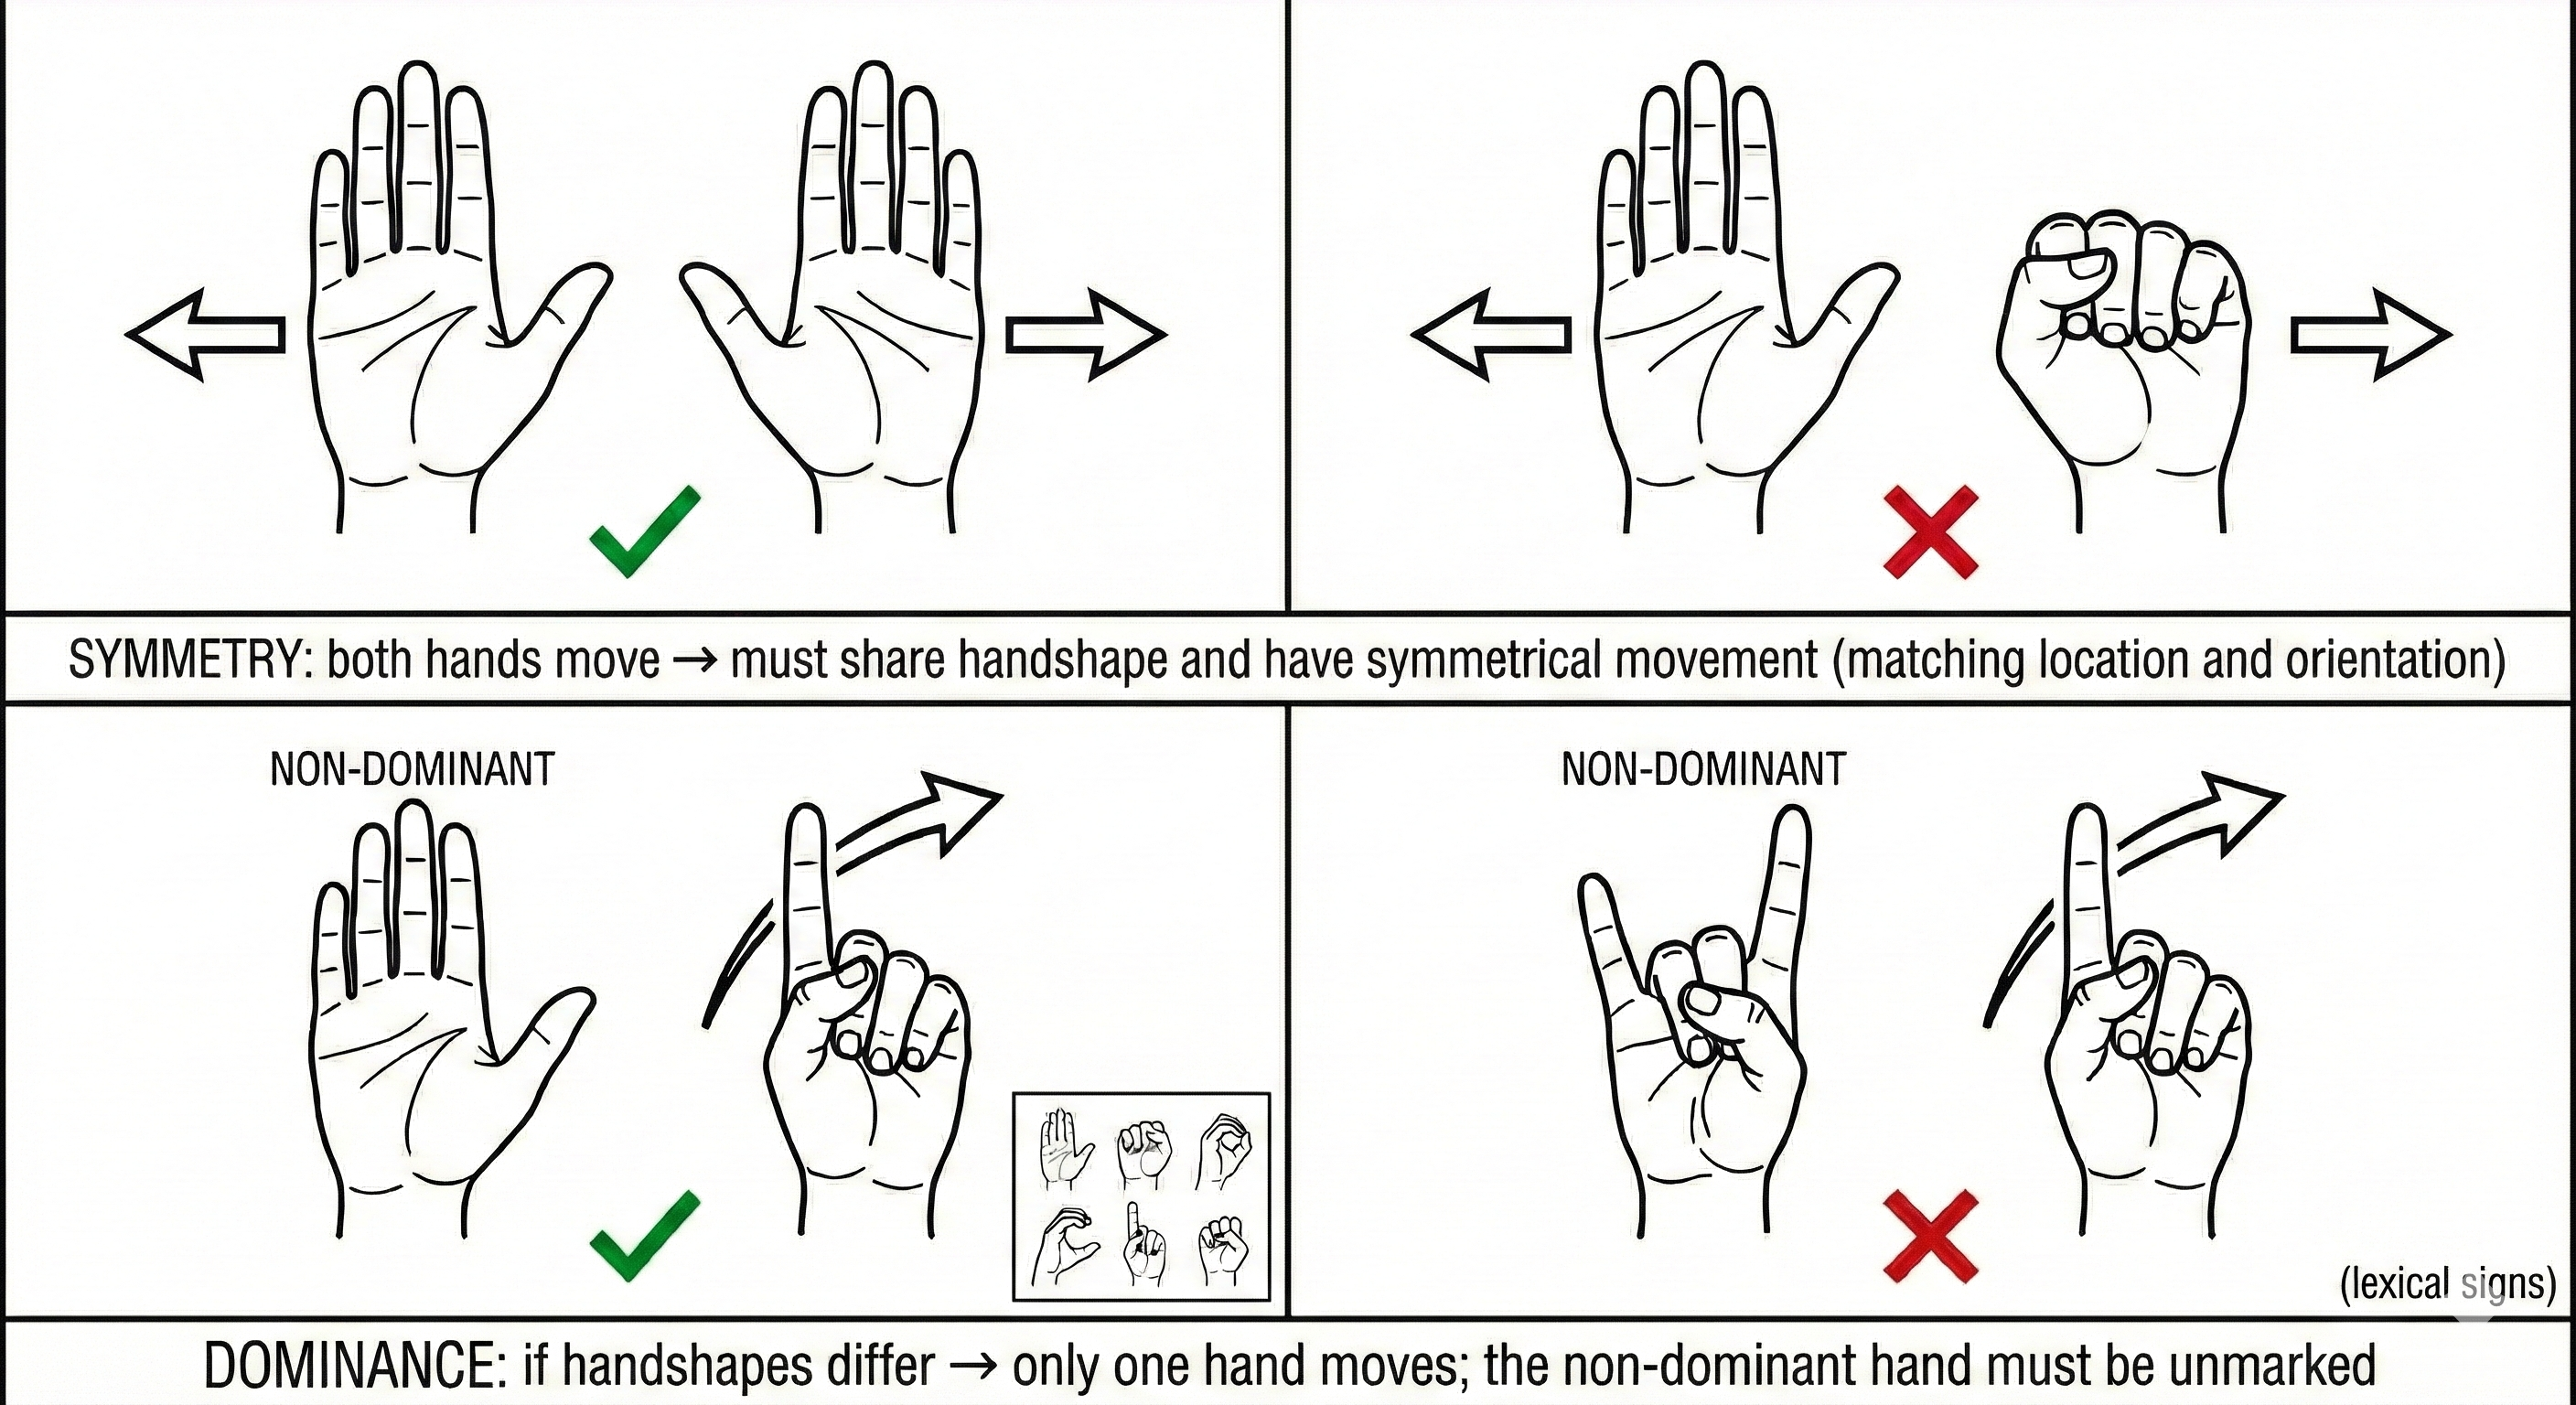
\includegraphics[width=0.85\textwidth]{figures/4.hands.png}
\caption{Phonological constraints in sign languages. Top: the symmetry condition requires that if both hands move, they share handshape and mirror each other's movement. Bottom: the dominance condition requires that if handshapes differ, only one hand moves, and the non-dominant hand uses an unmarked handshape. These constraints emerge independently across unrelated sign languages.}
\label{fig:sign-constraints}
\end{figure}

Nicaraguan Sign Language (NSL; Spanish acronym ISN) offers near-experimental evidence. NSL emerged in the late 1970s when deaf children were brought together in Managuan schools; no prior sign language was available as a model. Within two generations, NSL developed combinatorial phonology~-- discreteness, duality of patterning, minimal pairs~-- from holistic gestures \citep{senghas2004,senghas2005}. The mechanisms were visible in real time: children segmented continuous gestures into discrete components, regularized variation, imposed categorical structure. Phonological organization wasn't inherited; it was constructed by the same pressures that maintain it elsewhere.

Al-Sayyid Bedouin Sign Language (ABSL) in Israel confirms the pattern. \citet{sandler2011} found that Battison's symmetry and dominance constraints were absent in first-generation ABSL~-- signers freely combined handshapes without systematic constraints. But over three generations, as the language became more conventional, those constraints emerged. The structural regularities weren't inherited from another sign language; they crystallized from the same cognitive and motor pressures that produced them elsewhere.

This suggests the mechanisms maintaining phonological categories are more abstract than vocal-tract physics: categorical perception, motor-planning efficiency, perceptual distinctiveness under noise, learnability across generations \citep{emmorey2002}. These mechanisms operate over whatever articulatory-perceptual channel is available. The substrate varies; the clustering persists. This is HPC in action: different physical realizations, analogous mechanisms, convergent structure.


The framework doesn't need all groupings to be HPC kinds. Recall that I reserve \term{category} for mechanism-maintained kinds (§\ref{sec:2:where-essentialism-works}); what fails to meet that standard is a \term{class}~-- a label without the causal structure to back it up. Some classes might be thin~-- lacking the stabilizing mechanisms to produce robust clustering, like nonce coinages or idiolectal forms that never diffuse. Some might be fat~-- pooling heterogeneous phenomena under a single label, like cross-linguistic umbrellas that obscure distinct mechanisms. Some might be negative~-- mere complements, wastebasket classes defined by what they're not. Part of the work, going forward, is identifying which grammatical categories are which. Chapter~\ref{ch:failure-modes} develops criteria for diagnosis.


\section{How determinacy survives}
\label{sec:4:determinacy}

A worry hangs over the maintenance view: if categories don't have definitions, how can category membership be determinate? Isn't this just nominalism with extra steps~-- the view that categories are fictions, not facts?

The worry rests on a conflation. Determinacy doesn't require definitions; it requires causal grounding. A tiger is determinately a tiger not because it satisfies a checklist but because of its lineage~-- its causal-historical connection to other tigers, the mechanisms of reproduction and development that produced it. The same goes for linguistic categories. A word is determinately a noun not because it satisfies a definition but because the mechanisms that maintain \term{noun} have operated on it: it was acquired as a noun, used as a noun, aligned with other nouns, transmitted as a noun.

This is Millikan's point about proper functions \citep[ch.~1]{millikan1984}. An item's category membership is fixed by its history of production and use~-- by what mechanisms brought it into being and what mechanisms maintain it~-- not by what features it currently displays. The features matter because they're typically produced by the mechanisms. But when history and features diverge, history wins. A malformed tiger~-- one lacking stripes, say~-- is still a tiger because of its lineage. A malformed noun~-- one lacking typical nominal features~-- might still be a noun because of how it was acquired and used.

Where does indeterminacy arise? Where the causal pressures are genuinely mixed or transitional. Some items are hard cases not because we lack a definition to apply but because the mechanisms have been pulling in different directions: acquired as a noun but used increasingly like an adjective, with entrenchment patterns that are genuinely intermediate. The indeterminacy is real, but it's localized~-- a fact about this item in this transitional state~-- not a global fuzziness that infects the whole category.

Compare: are the Larus gulls circling the Arctic a single species or many? As you move around the ring~-- from Britain through Scandinavia to Siberia to Alaska to California~-- each population interbreeds with its neighbours. But the endpoints don't: herring gulls and lesser black-backed gulls, meeting in Britain, behave as distinct species. The mechanisms that maintain \mention{species}~-- reproductive isolation, morphological clustering, ecological niche~-- are strong at the endpoints and weak at the contact points. The indeterminacy is real, but it's localized to the transitions. No one doubts that robins and eagles are distinct species; the ring species are hard cases precisely where the mechanisms are in tension.

The same will be true for linguistic categories. Most nouns are determinately nouns; most verbs are determinately verbs. The core is stable because the mechanisms maintain it robustly. The periphery is where indeterminacy lives~-- and that's not a problem for the framework; it's a prediction.


\section{Recovering Aristotle}
\label{sec:4:aristotle}

Aristotle has had a longer career as a caricature of essentialism than as a guide to how kinds actually persist. But as §\ref{sec:2:what-essentialism-built} noted, real Aristotle was subtler. His essences weren't arbitrary definitions; they were supposed to be explanatory. The form of a thing explained its behaviour; the essence was what made the thing the kind of thing it was.

HPC recovers this insight. The homeostatic mechanisms are, in a sense, the essence~-- causally understood. What makes a tiger a tiger is the network of properties maintained by reproduction, development, and selection. What makes a noun a noun is the network of properties maintained by acquisition, entrenchment, alignment, and transmission. The mechanism-cluster \emph{is} the essence, relocated from the definitional to the causal register.

This is why HPC is sometimes called neo-Aristotelian \citep{boyd1999,wilson1999}. It recovers the structure Aristotle wanted~-- real natural kinds with genuine explanatory power~-- without the metaphysical baggage that made classical essentialism untenable. The kinds are real because they support induction. The induction works because the mechanisms maintain the clustering. The clustering is stable because the mechanisms are ongoing. It's a circle, but a virtuous one: mechanisms maintain clusters, and clusters sustain the mechanisms that maintain them.

The recovery isn't complete. Aristotle wanted essences to be intrinsic~-- properties a thing has independently of its relations to other things. HPC kinds are essentially relational: a tiger is a tiger because of its relations to other tigers (lineage), its relations to its environment (selection), its relations to developmental pathways (constraint). Linguistic categories are even more relational: a noun is a noun because of its relations to other nouns (analogy), its relations to speakers (acquisition, entrenchment), its relations to discourse (function). The essentialism being recovered is relational essentialism, not intrinsic essentialism.

That's a feature, not a bug~-- if the phrase itself is a bit prefab, that's fitting, because it trades on the same kind of relational uptake I'm describing. Linguistic categories are inherently relational~-- defined by distribution, opposition, system role. An account that makes them intrinsic would be false to what they are. HPC captures their relational nature while preserving their reality. The categories are real \emph{because} they're relational~-- maintained by relations that keep properties clustered.

A related objection runs deeper. Some philosophers have argued that species are not kinds at all but historical individuals~-- entities with spatiotemporal boundaries rather than classes with members \citep{ghiselin1974,hull1978}. On this view, \mention{tiger} names something more like a scattered object extended through space and time than a category with instances. The distinction matters for some purposes. But individuals, too, are maintained: what makes this tiger \emph{this tiger} over time is not an essence but a cluster of properties held in place by metabolic, developmental, and ecological mechanisms. The HPC question~-- what mechanisms maintain the clustering?~-- applies to individuals as well as to kinds. The species-as-individuals move doesn't escape the maintenance framework; it relocates within it.


\section{What \enquote{maintenance} commits us to}
\label{sec:4:maintenance-commitments}

By the end of Chapter~\ref{ch:what-we-havent-been-asking}, the slogan may sound almost disarmingly simple: categories are real because they are maintained. But the phrase \enquote{maintained} can hide either a substantive commitment or a decorative one. The substantive version says: there are identifiable processes that (i) keep certain properties co-occurring, (ii) stabilize those co-occurrences against perturbation, and (iii) thereby support reliable induction. The decorative version says: things seem stable, so let us call them maintained. The difference is the difference between explanation and renaming.

Homeostatic property cluster theory was never meant as a license for the decorative version. Boyd introduced HPC kinds to capture a familiar pattern in the sciences: kinds that are not definable by necessary and sufficient conditions, and yet are not mere human conveniences either, because their property clusters are held together by causal mechanisms \citep{boyd1991,boyd1999}. The mechanisms do not police membership by checking a definition. They make certain constellations more likely to occur and to persist, and those constellations are the basis for projection.

Recall the HPC commitment from page~\pageref{ch:kinds-without-essences}: a category is real when it is associated with a robust property cluster and there exist processes that tend to produce and stabilize that cluster. The point of formulating it this way was to make it vulnerable. It can fail: the cluster can be too thin to support induction; the apparent cluster can be an artefact of measurement; or the cluster can be real but maintained by multiple distinct processes, in which case the label covers several kinds rather than one. Those are empirical diagnoses that will matter later (Chapter~\ref{ch:failure-modes}).

\subsection{Mechanisms are not metaphors}
\label{subsec:4:mechanisms-not-metaphors}

In linguistic contexts, \enquote{mechanism} can sound like a promissory note: a way of gesturing at explanation while postponing it. Here it is meant as a constraint on what counts as an answer. If a category is maintained, then there must be identifiable points at which pressure can be applied and outcomes predicted. Perturbation should not merely produce change; it should produce \emph{structured} change.

The mechanisms appealed to in this book are heterogeneous in the mundane way that linguistic reality is heterogeneous. Some operate within an individual life (acquisition, entrenchment, alignment). Some operate across generations (iterated transmission). Some are neither purely individual nor purely social, because communicative function spans both: it shapes what is worth expressing and thus what survives learning and use. The mechanisms are not a finished list; they are the current best candidates for processes that are independently motivated and measurable.

Their shared role is not to define categories but to stabilize a landscape: to make some regions of grammatical space \emph{attractive} and others \emph{repellent}. A learner exposed to a community does not simply store tokens; they are pulled toward community-level regularities. A speaker in interaction does not merely express an idiolect; they coordinate. A system reproduced through imperfect learning does not simply degrade; it tends to reorganize into forms that pass more easily through the learning bottleneck. Taken together, these processes do not enforce crisp boundaries. They produce stability with seams, and discreteness with edge effects.

That is why boundary cases are not annoyances; they are probes. Culicover's \textit{Syntactic Nuts} makes the methodological point plainly: the places where classifications strain are often the places where the causal story is visible \autocite*{culicover1999}. If categories are maintained, then they should fail in characteristic ways under characteristic pressures. A framework that treats boundary cases as mere noise has surrendered the only data that can discriminate mechanisms.

\subsection{Comparative concepts revisited}
\label{subsec:4:comparative-concepts-revisited}

Haspelmath's insistence that cross-linguistic labels are \term{comparative concept}s has a force that an HPC view must respect. If typological categories were simply \emph{read off} from minds, the widespread mismatch between diagnostic criteria across languages would be mysterious. Comparative work does require yardsticks, and yardsticks are constructed \citep{haspelmath2010}.

But the crucial question is not whether the yardstick is constructed. It is whether the yardstick is \emph{responsive}: whether it tracks a cluster that is supported by mechanisms operating in the systems being measured. The difference matters because it bears on induction. A purely stipulative yardstick can be useful for bookkeeping, but it will not reliably support the generalisations linguists actually want: that phenomena grouped under one label will behave similarly under new tests, shift similarly under perturbation, and correlate with other properties in stable ways.

On the HPC view, the reality of a cross-linguistic category is not a claim that speakers everywhere represent \textsc{gender} or \textsc{number} in the same format. It is a claim that, despite heterogeneity of exponence and local organization, certain clusters recur because similar pressures tend to generate and stabilize them. Where the pressures differ, the clusters should not merely look different; they should come apart in diagnostic ways. Where the label survives such pressure-testing, it earns its keep as more than a filing device.

This reframes the nominalist's challenge. The nominalist is right that definitions fail. The nominalist is also right that categories can be useful without being essences. What the nominalist declines to ask is whether some useful categories are useful \emph{because} they track robust structure in the world---structure that can be discovered, tested, and sometimes revised. The HPC framework makes that question substantive rather than rhetorical.

\subsection{From maintenance to discreteness}
\label{subsec:4:from-maintenance-to-discreteness}

A remaining worry is that the HPC picture still sounds too continuous. If properties cluster because of graded pressures, why should the outcome not be merely graded as well? Why do linguistic categories \emph{feel} discrete even when their substrates are not?

This is not a side question. It is the point at which essentialism earns its intuitive appeal. Speakers routinely treat category membership as all-or-nothing: a sentence is grammatical or it is not; a word in a given use is a preposition or it is not; a sound is heard as /\ipa{ɪ}/ or /\ipa{ɛ}/ even when the acoustic signal varies continuously. If a non-essentialist realism can't say where such discreteness comes from, it will look like it has traded ontological seriousness for a tasteful shrug.

The next chapter takes up that problem directly. The shift in analogy there is not a change of subject but a change of scale. Biology supplies the picture of kinds without essences; physics supplies a clean model of how categorical outcomes can emerge from continuous substrates without any policing definition. Phase transitions are not introduced as a metaphor for language, but as a proof of concept: systems can have real, projectible categories whose sharpness is a dynamical achievement, not an intrinsic essence.

That is the handoff. If categories are maintained, then their boundaries must be maintained too. And if boundaries are maintained, we can ask what kind of sharpness a maintained boundary can have---sharp in structure, yet difficult to locate; stable under ordinary perturbations, yet sensitive near the seam. Chapter~\ref{ch:dynamic-discreteness} argues that this is exactly what we should expect, and shows how to make the expectation precise enough to test.

\subsection{If the maintenance view is wrong}
\label{subsec:4:falsification}

The claim isn't merely that categories are stable; it's that the stability is produced by mechanisms that can be identified, perturbed, and tracked. That claim has teeth.

If the maintenance view is wrong, here is what we should observe: category boundaries should not respond predictably to perturbations that target specific mechanisms. Shift acquisition patterns~-- change the distributional signatures in child-directed speech~-- and boundary locations should remain fixed if the mechanisms are epiphenomenal. Shift register distributions~-- flood a construction with informal-written tokens via online discourse~-- and the category should stay put if alignment is decorative. Shift transmission dynamics~-- isolate a community or introduce contact~-- and the clustering should be unaffected if iterated learning does no real work.

We should also fail to find the variance signature: distance-to-boundary should not predict judgment spread. If boundaries are brute rather than maintained, there is no reason for items near them to show heightened variance; the instability is unmotivated.

Conversely, if the maintenance view is right, the research programme writes itself. For each mechanism, identify a perturbation; predict a direction and timescale of shift; measure. The \mention{fun} case is the cleanest available exemplar: register shift toward informal written + alignment in online discourse predicts faster adjectivalisation; diachronic corpus data should show boundary movement and, eventually, reduced variance once entrenchment catches up. That is the kind of prediction the framework is designed to generate.
